%%%%%%%%%%%%%%%%%%%%%%%%%%%%%%%%%%%%%%%%%%
\chapter{Packed Bed Heat Transfer} \label{ch:heat-transfer}
%%%%%%%%%%%%%%%%%%%%%%%%%%%%%%%%%%%%%%%%%%
[talk about how lacking the DEM result is without the inclusion of helium in analysis. There are some Fusion papers on conductivity in vacuum and with helium]

We now consider the influence of helium on thermal transport of deposited nuclear energy as it is carried away by the cooled structural walls. We begin by considering the fluid in a continuum sense and the pebbles in a discrete one. The interactions of the fluid and solid are characterized by effective relationships in each discretized cell of fluid. We then consider an mesoscopic approach to the fluid-solid interaction with the Lattice-Boltzmann method. 

The chapter begins with introduction of the coupled fluid dynamics - discrete element method (CFD-DEM) approach: governing equations, discretization techniques, and algorithms.

We then do LBM. And stuff.

%%%%%%%%%%%%%%%%%%%%%%%%%%%%%%%%%%%%%%%%%%
\section{Single particle heat transfer}

\begin{figure}[t]
	\centering
	\caption{Each ceramic pebble in a fusion reactor will experience multiple modes of heat transfer.}
	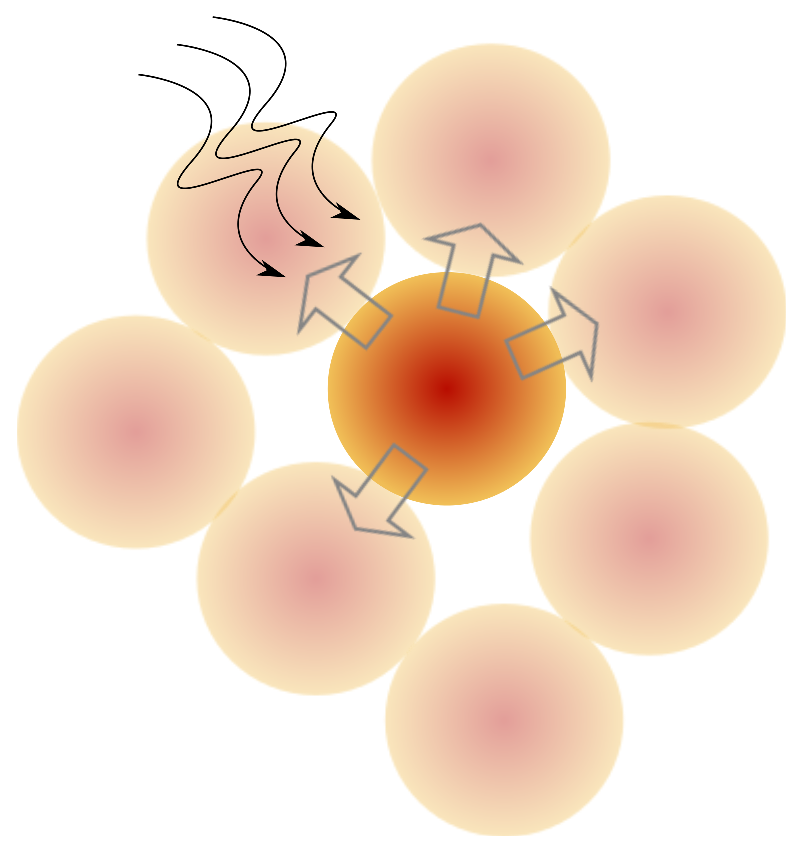
\includegraphics[width=0.75\textwidth]{chapters/figures/pebble-complete-heat-transfer}\label{fig:peb-comp-ht}
\end{figure}

Shown in Fig.~\ref{fig:peb-comp-ht} are all the modes of energy transfer on a pebble inside the fusion reactor. There is:

\begin{enumerate}
\item energy generated internal to the pebble caused by nuclear heating,
\item conduction internally of the solid material to the surface of the pebble, 
\item conduction between neighboring pebbles at their areas of contact, 
\item radiation between neighboring solids, and 
\item convective heat transfer with the interstitial helium gas (which includes energy carried far downstream or redeposited to neighboring pebbles).
\end{enumerate}









\subsection{Nuclear heating}

Nuclear deposition of energy is handled in a straightforward manner in the DEM computations with a simple source term on the energy balance equation. 












\subsection{Conduction through the solid}\label{sec:ht-pebble-conduction}

Before considering the heat equation in a sphere, it is instructive to first consider the simpler problem of a one-dimensional slab with volumetric heat generation, $q_g'''$ and convective cooling at the surfaces. The geometry is shown in Fig.~\ref{}.

Assuming we can find the Nusselt number for the convective cooling, we write the heat flux from the surface to the fluid as

\begin{equation}
	q_s'' = h(T_s - T_f)	
\end{equation}

where $T_f$ is the bulk fluid temperature and $T_s$ is the surface temperature. At steady-state the amount of heat moved across the fluid-surface interface must necessarily be equal to the total amount of heat generated into the slab. Therefore,

\begin{equation}
	q_w'' = q_g'''L = h(T_f-T_s)
\end{equation}

where $L$ is the half-width of the slab. For the sake of discussion, we re-write the above in terms of the temperature delta from surface to fluid in terms of nuclear heating,

\begin{equation}\label{eq:fluid-delta}
	T_f-T_s = \frac{q_g'''L}{h}
\end{equation}

Inside the slab, at steady-state the energy equation is simply a balance of heat conduction and nuclear generation. 

\begin{equation}\label{eq:nuclear-heating-slab-ode}
	0 = k\frac{\mathrm{d}^2T}{\mathrm{d}x^2} + q_g'''
\end{equation}

The boundary conditions are symmetry about the centerline and known surface temperature

\begin{align}
	q_{L=0} &= 0 \\
	T(L) &= T_s
\end{align}

The ODE of Eq.\ref{eq:nuclear-heating-slab-ode} is solved with simple separation and integration. When the boundary conditions are applied we have

\begin{equation}
	T(x) = \frac{q_g''' L^2}{2k}\left(1-\frac{x^2}{L^2}\right) + T_s
\end{equation}

We can find the temperature at the centerline of the slab, $x = 0$ as

\begin{equation}
	T_{cl} = \frac{q_g''' L^2}{2k} + T_s
\end{equation}

Or,

\begin{equation}\label{eq:centerline-delta}
	T_{cl} - T_s = \frac{q_g''' L^2}{2k}
\end{equation}

From Eqs.~\ref{eq:fluid-delta} and~\ref{eq:centerline-delta}, we see that the temperature differences between the surface and the fluid or the centerline and the surface are dictated by the heat generation rate relative to the speed at which that heat can be transported, via convection or conduction, respectively.

We will divide Eq.~\ref{eq:centerline-delta} by Eq.~\ref{eq:fluid-delta},

\begin{equation}\label{eq:biot-derivation}
	\frac{T_{cl} - T_s}{T_f-T_s} = \frac{1}{2}\frac{hL}{k}
\end{equation}

Careful observation of this equation can tell us much about the relative importance of the different modes of heat transfer to/from the surface. If the thermal transport away from the surface occurs at a much slower pace than thermal transport of energy through the solid to the surface, then the change in temperature across the solid $T_{cl}-T_{s}$ will be small compared to the change in temperature from the interface of solid to the bulkd fluid temperature, $T_{s}-T_f$. If the temperature across the solid is negligibly small in comparison to the surface-fluid difference, we are safe in the assumption that the solid is isothermal.

The group of terms on the right-hand-side of Eq.~\ref{eq:biot-derivation} is recognized as the Biot number,

\begin{equation}\label{eq:biot-number}
	\Bi=\frac{hL}{k}=\frac{R_{cond}}{R_{conv}}
\end{equation}

whose value is used to quantify the importance of internal conduction in the analysis of the solid interacting with convective heat transfer. If $\Bi<<1$, it is safely assumed that there is no temperature gradient in the solid material. A conclusion that will prove helpful in later analysis.

It is interesting to note that in this derivation of Biot number, we had considered nuclear heating as the source for temperature gradients across the pebble yet the rate of nuclear heating still does not appear in the Biot number. This implies that traditional assumptions of the validity of the lumped capacitance method hold even when dealing with a heat generation term in our energy balance.





\subsubsection{Large Biot number}

As we saw from the discussion of Eq.~\ref{eq:biot-number}, when the Biot number is small we can safely neglect temperature gradients through the solid we are analzying. However, when dealing with materials with low conductivity, i.e. larger $\Bi$, this assumption of negligible temperature gradient becomes decreasingly valid.  When dealing with spheres, there are slighty different accepted definitions of the Biot Number.  Some suggest that $\Bi=hd_p/6k$ is acceptable\cite{incropera:245}, where $d_p$ is the diameter of the particle.  However many use the more conservative definition of $\Bi=hd_p/2k$\cite{incropera:245,jeffreson409}.  For consistency and conservatism, we will proceed here with the latter definition.  

Considering now material and geometric properties relevant to our ceramic pebble beds, we will see that we may need to consider the effects of a larger $\Bi$ for our pebbles. The helium purge gas moving through the packed beds is not specifically intended to act as a heat transfer agent and moves along at a creeping flow rate. For a first approximation we will therefore assume as a lower limit the Nusselt number is $\Nu = 2$ (the value for a sphere in quiescent fluid). From the requirement that $\Bi \ll 1$, we have

\begin{equation}
	2 \frac{k_f}{k_s} \ll 1
\end{equation}

The conductivity of helium over the temperature range of 300 to 800 $^\circ$C is approximately 0.3 \si{W/m-K}. The solid conductivity of \lit and \lis are approximately 2 \si{W/m-K}. Because of the low conductivity of our solid, the Biot assumption is barely valid, $0.3 < 1$. 


































[Go back through Batchelor and O'Brien~\cite{Batchelor1977} paper]

\begin{equation}
	\frac{ k_s }{ k_f } \frac{a}{R^*} = \lambda
\end{equation}

Similar to the lumped capacitance assumptions, if $\lambda \gg 1$, the solid is approximately is isothermal. The second group on the left-hand side of this condition we remember from the assumptions of Hertz theory, where we require $\frac{a}{R^*} \ll 1^*$. Therefore to satisfy the condition of $\lambda \gg 1$, we require very large conductivity ratios of solid to fluid, $\frac{k_s}{k_f} \gg 1$. Alternatively this is satisfied by definition if the solids exist in vacuum.

Assuming that we satisfy the condition of isothermal solids, we address the conduction between solids in their small regions of contact.

[more details]










\subsection{Particle-particle conduction}

Handling the heat transfer between contacting particles has been investigated extensively by researchers in a number of fields\cite{Zhou2009,Zhang2011,Wu2011,Vargas2001,Li2000,Chaudhuri2006}. The amount of energy per time that can be transported per difference in temperature between pebble $i$ and $j$ as a conductance $h_{ij}$. Defined as

\begin{equation}\label{eq:pebble-conductance}
	\frac{h_{ij}}{k^*}= 2\left[\frac{3F_nR^*}{4E^*}\right]^{1/3}
\end{equation}

$k^*= 2k_ik_j/(k_i+k_j)$ is the effective solid conductivity of the two particles, and $F_n$ is the magnitude of the normal force between particles $i$ and $j$ as calculated by Eq.~\ref{eq:hertzForce}. Therefore, if we consider particles at temperatures $T_i$ and $T_j$ in contact, they will transfer heat at a rate of

\begin{equation}
	Q_{ij} = h_{ij}(T_i - T_j)
\end{equation} 











\subsection{Convection}











\subsection{Particle-particle radiation}
\section{Jeffreson correction to lumped capacitance method}\label{sec:ht-jeffreson-correction}
In \S\ref{sec:particle-convection}, we discuss correlations for heat transfer coefficients of spheres in a packed bed. Then those correlations are utilized with CFD-DEM computational routines in \S\ref{eq:cfdem-dem-energy}. When implemented in the DEM-based modeling, we make the lumped capacitance assumption for each particle in the ensemble. The assumption eases the computational efforts of solving for the temperature distribution inside each particle; each particle is treated as isothermal. The accuracy of the lumped capacitance method is described by the Biot number,

\begin{equation}
     \Bi = \frac{hd_p}{k_r}
\end{equation} 

and for $\Bi \ll 1$ the lumped capacitance method accurately models the behavior of a solid interacting with a fluid. For $\Bi \approx 0.1$, the error from the lumped capacitance method is only about 5\%. In solid breeder volumes, the particles are generally small, solid conductivity low, and heat transfer coefficient generally also low. This leads to small-to-moderate Biot numbers expected in the packed bed. In this section we will analyze the accuracy of the lumped capacitance and introduce a correction method to account for inaccuracies of the method at moderate Biot numbers.

We simplify the case of a packed bed and only consider a single sphere with volumetric heat generation submerged in and thermally interacting with a fluid. The sphere will be of radius $R=d_p/2$, as shown in Fig.~\ref{fig:ParticleControlVolume}. The sphere will initially be at a uniform temperature of $T_i$. The fluid temperature will remain constant at $T_f$

\begin{figure}[ht]
	\centering
		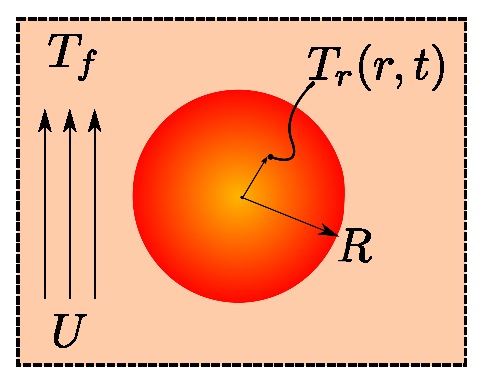
\includegraphics[width=2in]{chapters/figures/ParticleControlVolume}
	\caption[Control volume of single spherical particle in a packed bed]{CONTROL VOLUME OF A SINGLE SPHERICAL PARTICLE IN A PACKED BED}
	\label{fig:ParticleControlVolume}
\end{figure}


%~~~~~~~~~~~~~~~~~~~~~~~~~~~~~~~~~~~~~~~~~~~~~~~~~~~~~~~
\subsection{Lumped capacitance solution for sphere}\label{sec:lumped-capacitance}
We will solve for a single sphere interacting with a passing fluid, as shown in Fig.~\ref{fig:ParticleControlVolume}. We make the lumped capacitance assumption for this sphere. The solid is initially at temperature $T_0$, with constant volumetric heat generation, cooling in a fluid with constant heat transfer coefficient. The fluid will remain constant at $T_f$.

The time response of the sphere's temperature is dictated by the balance of energy to/away from the solid,  

\begin{equation}\label{eq:lc-energy-balance}
	\rho_rC_rV\frac{dT}{dt} = -hA(T-T_f) + gV
\end{equation}

Eq.~\ref{eq:lc-energy-balance} is solved in dimensionless form with the following nondimensional parameters of temperature and time,

\begin{subequations}
\begin{align}
    \theta &= \frac{T(t) - T_f}{T_0 - T_f}\\
    \tau & = \frac{t}{R^2/\alpha}
\end{align}
\end{subequations}

where $\alpha$ is the thermal diffusivity of the sphere, $T_0$ is the initial isothermal temperature of the sphere, and $T_f$ is the constant fluid temperature. The resulting temperature distribution is,

\begin{equation}
\label{eq:theta-lc}
	\theta_{LC}=\left(1-\frac{G}{3\Bi}\right)\exp(-3\Bi \tau) + \frac{G}{3\Bi}
\end{equation}

where we define a dimensionless heat generation,

\begin{equation}\label{eq:nondimensional-heat-generation}
	G = \frac{gR^2}{k(T_0 - T_f)}
\end{equation}

The energy of the sphere, relative to the fluid, in nondimensional terms is 

\begin{equation}
    E^*(\tau)=\frac{E(\tau)}{E_0}
\end{equation}

where $E_0$ is the initial energy of the sphere,

\begin{equation}
    E_0=\rho_rC_rV(T_0-T_f)
\end{equation}

Thus for a sphere with the lumped capacitance model, in nondimensional form, is simply

\begin{equation}\label{eq:lc-energy-profile}
	E^*_{LC}(\tau) = \theta_{LC}(\tau)
\end{equation}

The nondimensional energy profile of Eq.~\ref{eq:lc-energy-profile} is plotted over the nondimensional time of $\tau \in [0,1/\Bi]$ in Fig.~\ref{fig:LC-sphere-in-fluid}. 

\begin{figure}[ht]
	\centering
		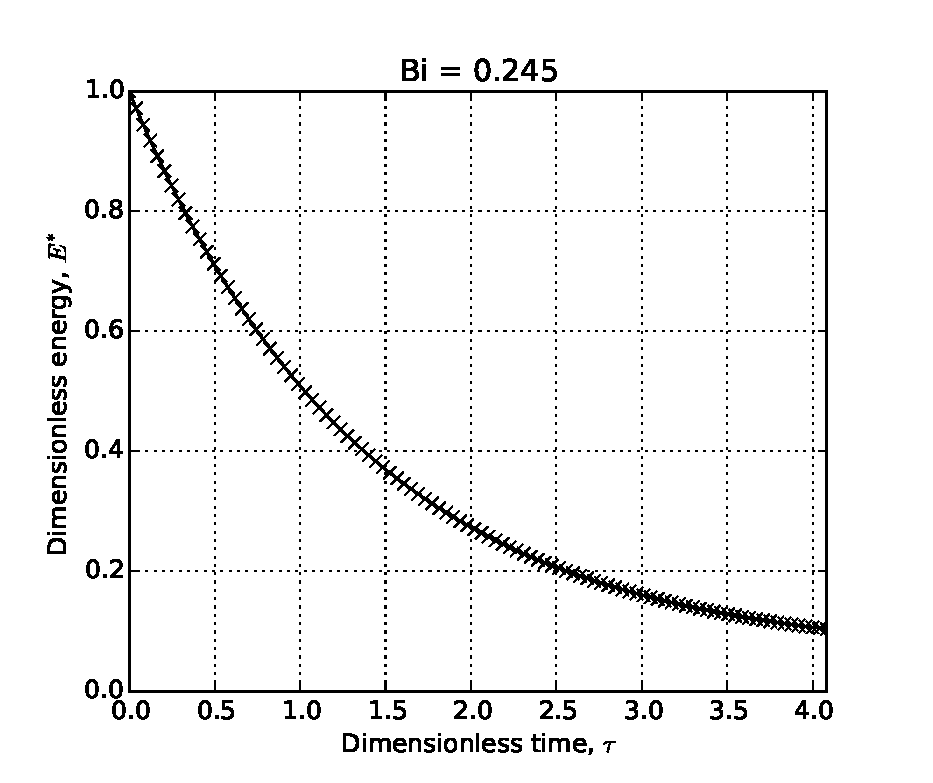
\includegraphics[width=0.75\textwidth]{chapters/figures/LC-sphere-in-fluid}
	\caption[Lumped Capacitance energy profile]{Lumped capacitance model: Sphere energy profile decaying from an initial value to a time of $1/\Bi$}
	\label{fig:LC-sphere-in-fluid}
\end{figure}

Reviewing Eq.~\ref{eq:theta-lc} we see that the speed of decay is dictated by the term in the exponential, $3\Bi$. Meanwhile, the steady-state value being approached is given by $\frac{G}{3\Bi} = \frac{gR}{h(T_0 - T_f)}$. It is important for this discussion to point out that because both the nondimensional heat generation and Biot number terms contain the solid conductivity, the steady-state value of the lumped capacitance model will not change for varying solid conductivity even if it leads to different Biot numbers. We will return to this point in the next section when we compare the lumped capacitance model to the exact solution when internal conduction of the solid is considered.
%~~~~~~~~~~~~~~~~~~~~~~~~~~~~~~~~~~~~~~~~~~~~~~~~~~~~~~~



%~~~~~~~~~~~~~~~~~~~~~~~~~~~~~~~~~~~~~~~~~~~~~~~~~~~~~~~
\subsection{Exact solution for sphere}\label{sec:analytic-sphere}

We again analyze the sphere of Fig.~\ref{fig:ParticleControlVolume} but now will account for internal temperature gradients inside the sphere. The details of the analytic solution for a sphere with heat generation interacting with a fluid is given in Appendix~\ref{sec:analytic-sphere-details}. We again solve in terms of the nondimensional temperature and time introduced in \S\ref{sec:lumped-capacitance} as well as a nondimensional radius,

\begin{align*}
    \theta &= \frac{\mathbb{T}}{\mathbb{T}_0}\\
    \rho & = \frac{r}{R}\\
    \tau & = \frac{t}{R^2/\alpha}
\end{align*}

The energy conservation equation for the sphere with internal temperature gradient, in nondimensional form $\theta_{TG}$, is

\begin{equation}
    \frac{1}{\rho}\frac{\partial^2}{\partial \rho^2}(\rho\theta_{TG}) + G = \frac{\partial\theta_{TG}}{\partial \tau}
\end{equation}

With the initial condition and boundary conditions outlined in Appendix~\ref{sec:analytic-sphere-details}, the nondimensional temperature distribution inside the sphere is 

\begin{equation}\label{eq:analytic-temperature-distribution}
    \theta_{TG}(\rho,\tau) = \left(\frac{G}{6} + \frac{G}{3\Bi}-\rho^2\right)  +   \sum_{n=1}^\infty \exp(-\zeta^2 \tau) \frac{\sin(\zeta_n \rho)}{\rho} \frac{Z(\zeta_n)}{N(\zeta_n)}  
\end{equation}

where $\zeta_n$ are the eigenvalues of the equation and the functions of $\zeta_n$ ($Z$,$N$,$C$) are given in Appendix~\ref{sec:analytic-sphere}. 

The accompanying nondimensional energy of the sphere is integrated to,

\begin{equation}
\label{eq:analytic-energy-profile}
    E^*_{TG}(\tau)=\left(\frac{G}{15}+\frac{G}{3\Bi}\right)+3\sum_{n=1}^\infty \exp(-\zeta^2 \tau) \frac{Z(\zeta_n)}{N(\zeta_n)} C_n(\zeta_n)
\end{equation}

We now compare the exact solution from Eq.~\ref{eq:analytic-energy-profile} to the solution of energy given by the lumped capacitance model of Eq.~\ref{eq:lc-energy-profile}. The two profiles are given in Fig.~\ref{fig:LC-analytic-sphere-in-fluid}. 

\begin{figure}[ht]
	\centering
		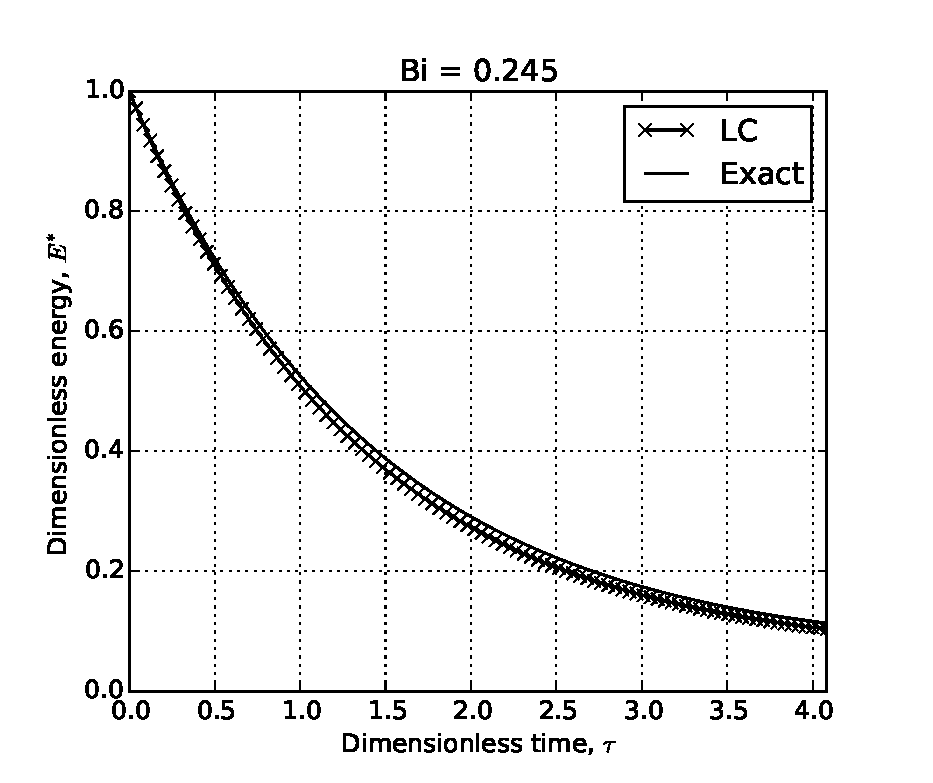
\includegraphics[width=0.75\textwidth]{chapters/figures/LC-analytic-sphere-in-fluid}
	\caption[Analytic temperature profile for $\Bi < 1$]{Analytic and lumped capacitance models: Sphere energy profile decaying from an initial value to a time of $1/\Bi$}
	\label{fig:LC-analytic-sphere-in-fluid}
\end{figure}

For the value of Biot number here, $\Bi < 0.5$, the profile of the analytic solution of the sphere is well-captured by the lumped capacitance model. The maximum relative error over the time span, as defined by

\begin{equation}\label{eq:error}
	\text{error} = \frac{\big|E^*_{TG}(\tau) - E^*_{LC}(\tau) \big|}{E^*_{TG}(\tau)}
\end{equation}

is always less than 10\%. 

We consider now the same size sphere but with the Biot number increased by an order by: a) a conductivity of $k = k_r/10$ and b) a heat transfer coefficient of $h = 10h_f$. The two physical changes to the system result in the same Biot number but as we can see in Fig.~\ref{fig:LC-analytic-sphere-in-fluid-Bi-2}, there are drastic changes in the results. 

\begin{figure}
        \centering
        \begin{subfigure}[b]{0.5\textwidth}
                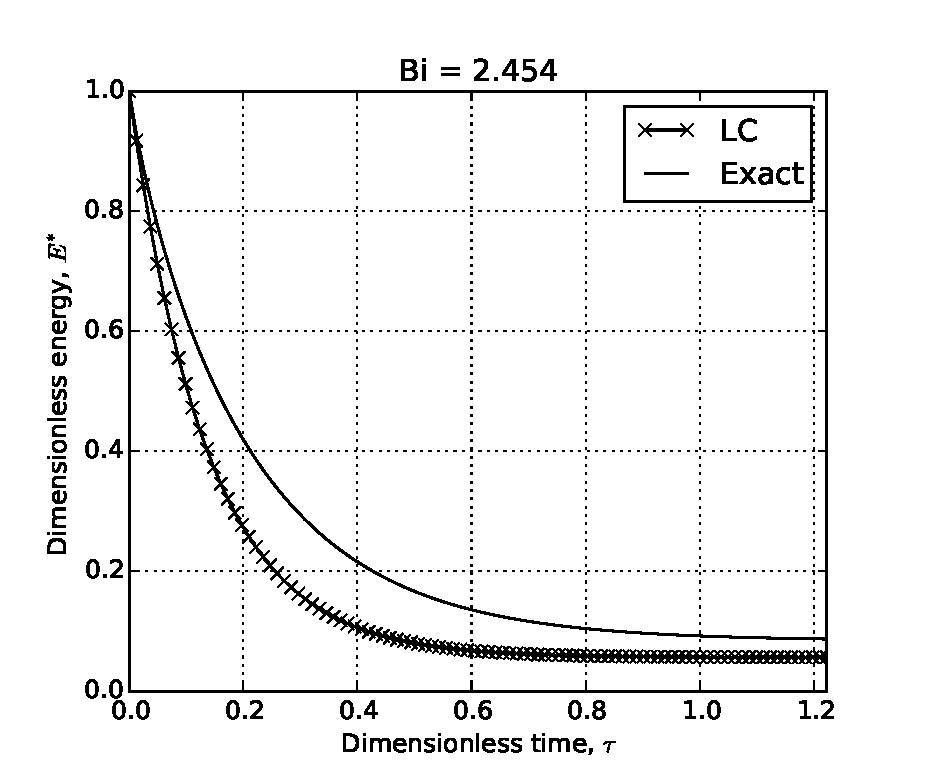
\includegraphics[width=\textwidth]{chapters/figures/LC-analytic-sphere-in-fluid-Bi-2a}
                \caption{The Biot number increased from a decrease in the solid conductivity.}
				\label{fig:LC-analytic-sphere-in-fluid-Bi-2a}
        \end{subfigure}%
        
          %add desired spacing between images, e. g. ~, \quad, \qquad, \hfill etc.
          %(or a blank line to force the subfigure onto a new line)
        \begin{subfigure}[b]{0.5\textwidth}
                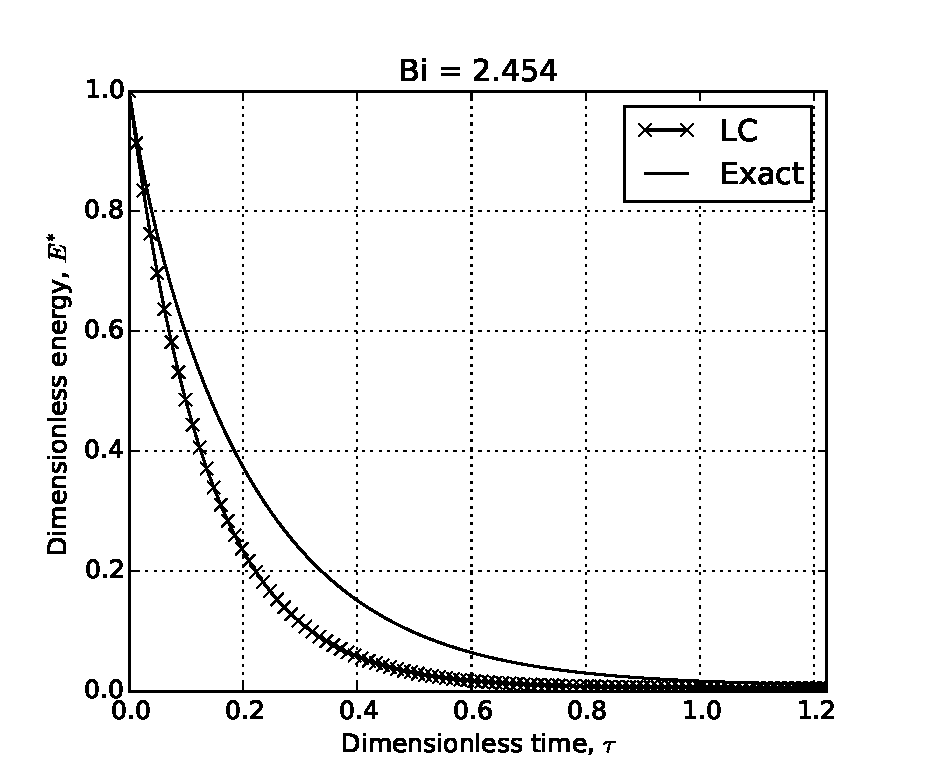
\includegraphics[width=\textwidth]{chapters/figures/LC-analytic-sphere-in-fluid-Bi-2b}
                \caption{The Biot number increased from  an increase in the heat transfer coefficient.}
				\label{fig:LC-analytic-sphere-in-fluid-Bi-2b}
        \end{subfigure}
        \caption[Analytic temperature profile for moderate Biot number]{Analytic and lumped capacitance models: Sphere energy profile decaying from an initial value to a time of $3/\Bi$. The same Biot number produces different results for the exact solution of a sphere with heat generation.}\label{fig:LC-analytic-sphere-in-fluid-Bi-2}
\end{figure}

Seen in Fig.~\ref{fig:LC-analytic-sphere-in-fluid-Bi-2a}, the lumped capacitance solution both over-predicts the speed at which the sphere reaches a thermal steady-state as well as the value of the steady-state. Comparatively, in Fig.~\ref{fig:LC-analytic-sphere-in-fluid-Bi-2b}, for the same Biot number the lumped capacitance solution again over-predicts the speed to thermal steady-state by the same rate but is relatively accurate for the steady-state value itself. 

To first address the source of error on the steady-state value, we view the steady-state terms of the two solutions. From Eq.~\ref{eq:analytic-energy-profile}, we write the steady-state term of the exact solution as 

\begin{equation}
	E^*_{TG,ss}=\frac{G}{15}+\frac{G}{3\Bi}
\end{equation}

Comparatively, we write the steady-state term of the lumped capacitance solution from \S\ref{sec:lumped-capacitance} as,

\begin{equation}
	E^*_{LG,ss} = \frac{G}{3\Bi}
\end{equation}

We clearly see that the two steady-state values differ by the contribution of $\frac{G}{15}$ on the exact solution. This term does not appear in the lumped capacitance solution because it does not account for the temperature difference through the sphere. The nondimensional heat generation term is given in Eq.~\ref{eq:nondimensional-heat-generation}; it is importantly a function of thermal conductivity but not the heat transfer coefficient. This explains the difference between steady-state values in Fig.~\ref{fig:LC-analytic-sphere-in-fluid-Bi-2} when we modified the two parameters.

To address the inaccuracies in the time-dependent response of the lumped capacitance method with large Biot number, we will make use of the so-called Jeffreson Correction described by Van Lew\cite{VanLew2010} and Xu et al.\cite{Xu2012}. In their work, they considered a heated heat transfer fluid interacting with a low conductivity thermal storage material. The solar thermal storage systems they analyzed often had moderate-to-large Biot numbers but they could continue to apply the lumped capacitance model by applying the Jeffreson Correction\cite{jeffreson409}. The details of the Jeffreson correction as applied to a system with volumetric heat generation will be discussed next.
%~~~~~~~~~~~~~~~~~~~~~~~~~~~~~~~~~~~~~~~~~~~~~~~~~~~~~~~





%~~~~~~~~~~~~~~~~~~~~~~~~~~~~~~~~~~~~~~~~~~~~~~~~~~~~~~~
\subsection{Jeffreson correction for sphere}
In Fig.~\ref{fig:LC-analytic-sphere-in-fluid-Bi-2}, the lumped capacitance model predicted a much faster decay to steady-state than the exact solution. Jeffreson summarized a correction to the lumped capacitance model via a reduction in the heat transfer coefficient as a function of the Biot number. The smaller heat transfer coefficient effectively slowed the decay to steady-state as predicted by the lumped capacitance method.
The correlation to correct the heat transfer coefficient due to solids with large Biot number is given by Jeffreson\cite{jeffreson409}. The Jeffreson correction for a sphere is,

\begin{equation}
	h_{p}=\frac{h}{1+\Bi/5}
\end{equation}

where $h_p$ is the modified heat transfer coefficient of the particle with an internal temperature gradient.  An increase in the Biot Number (or increase of thermal gradient inside the solid) results in a decrease in the heat transfer coefficient~$h_p$. A modified Biot number can then also be written as

\begin{equation}\label{eq:jeffreson-correction-bip}
	\Bi_p = \frac{h_p d}{k_r} = \frac{\Bi}{1+\Bi/5}
\end{equation}

Applying the Jeffreson Correction to Eq.~\ref{eq:theta-lc},

\begin{equation}
\label{eq:theta-jc-bip}
	\theta_{JC}=\left(1-\frac{G}{3\Bi_p}\right)\exp\left(-3\Bi_p \tau\right) + \frac{G}{3\Bi_p}
\end{equation}

and thereby Eq.~\ref{eq:lc-energy-profile} gives

\begin{equation}\label{eq:jc-energy-profile}
	E^*_{JC}(\tau) = \theta_{JC}(\tau)
\end{equation}

We then plot the energy profiles from the lumped capacitance model (LC), the Jeffreson correction (JC), and the exact solution together in Fig.~\ref{fig:LC-JC-analytic-sphere-in-fluid-Bi-2}

\begin{figure}
        \centering
        \begin{subfigure}[b]{0.5\textwidth}
                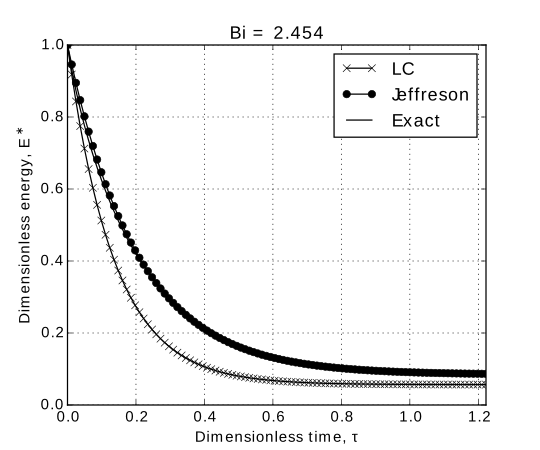
\includegraphics[width=\textwidth]{chapters/figures/LC-JC-analytic-sphere-in-fluid-Bi-2a}
                \caption{The Biot number increased from a decrease in the solid conductivity.}
				\label{fig:LC-JC-analytic-sphere-in-fluid-Bi-2a}
        \end{subfigure}%
        
          %add desired spacing between images, e. g. ~, \quad, \qquad, \hfill etc.
          %(or a blank line to force the subfigure onto a new line)
        \begin{subfigure}[b]{0.5\textwidth}
                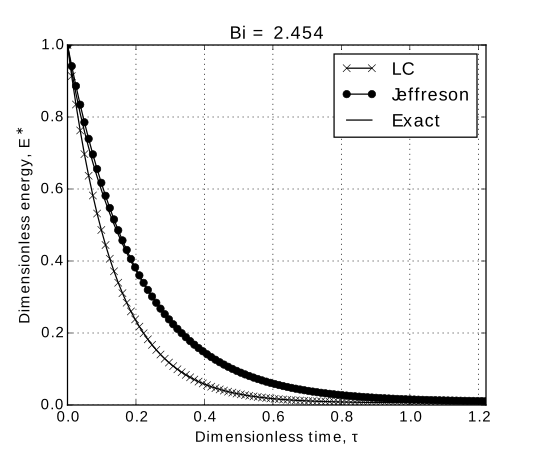
\includegraphics[width=\textwidth]{chapters/figures/LC-JC-analytic-sphere-in-fluid-Bi-2b}
                \caption{The Biot number increased from  an increase in the heat transfer coefficient.}
				\label{fig:LC-JC-analytic-sphere-in-fluid-Bi-2b}
        \end{subfigure}
        \caption[Jeffreson correction for moderate Biot number based on conductivity]{Analytic, lumped capacitance model, and LC model with Jeffreson correction: Jeffreson correction corrects for transient and steady-state errors of lumped capacitance.}\label{fig:LC-JC-analytic-sphere-in-fluid-Bi-2}
\end{figure}

The Jeffreson correction to the lumped capacitance method allows the simple model to capture the proper transient as well as steady-state values for this sphere with a moderately sized Biot number. To look more closely, we view the instantaneous error (see Eq.~\ref{eq:error}) in Fig.~\ref{fig:LC-JC-analytic-error-Bi-2}.

\begin{figure}
        \centering
        \begin{subfigure}[b]{0.5\textwidth}
                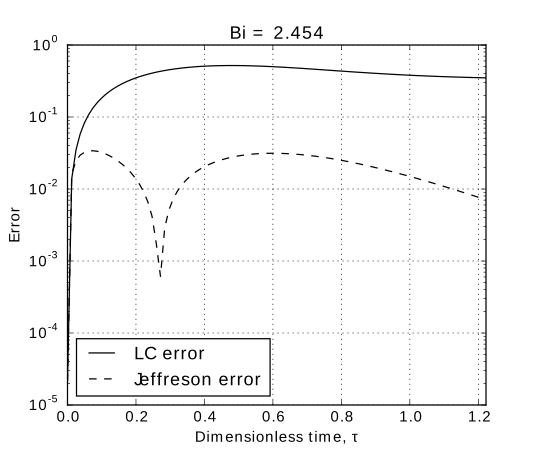
\includegraphics[width=\textwidth]{chapters/figures/LC-JC-analytic-error-Bi-2a}
                \caption{The Biot number increased from a decrease in the solid conductivity.}
				\label{fig:LC-JC-analytic-error-Bi-2a}
        \end{subfigure}%
        
          %add desired spacing between images, e. g. ~, \quad, \qquad, \hfill etc.
          %(or a blank line to force the subfigure onto a new line)
        \begin{subfigure}[b]{0.5\textwidth}
                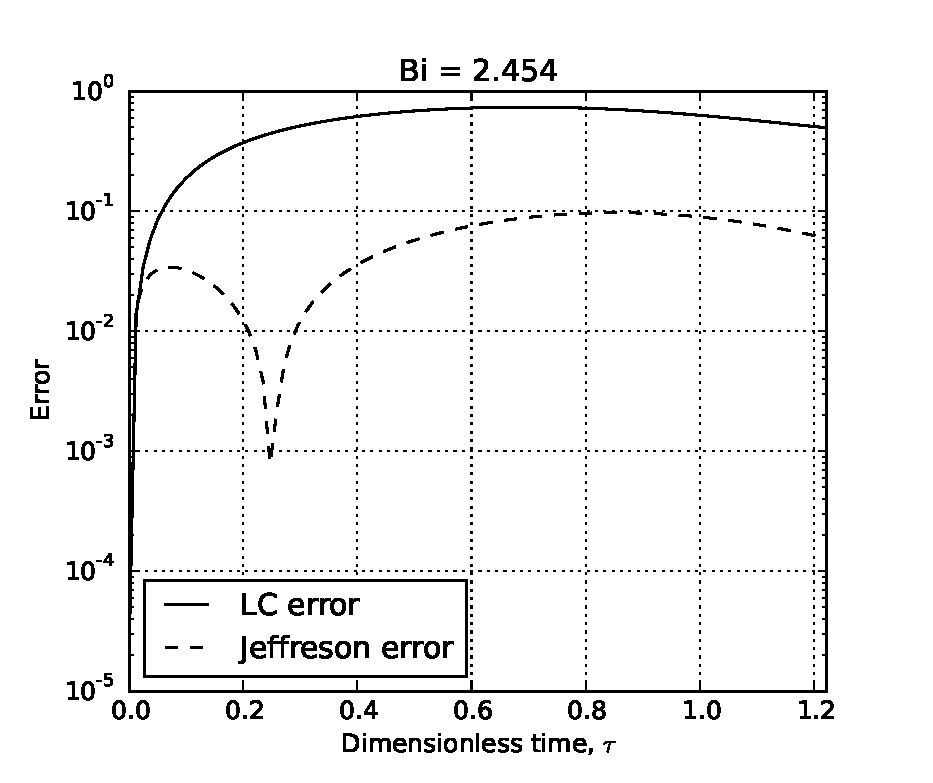
\includegraphics[width=\textwidth]{chapters/figures/LC-JC-analytic-error-Bi-2b}
                \caption{The Biot number increased from  an increase in the heat transfer coefficient.}
				\label{fig:LC-JC-analytic-error-Bi-2b}
        \end{subfigure}
        \caption[Error of lumped capacitance and Jeffreson correction for moderate Biot number]{Error of lumped capacitance and reduced error of the model with Jeffreson correction for moderate Biot number.}\label{fig:LC-JC-analytic-error-Bi-2}
\end{figure}

For the value of $\Bi > 1$ due to either low conductivity (Fig.~\ref{fig:LC-JC-analytic-error-Bi-2a}) or high heat transfer coefficient (Fig.~\ref{fig:LC-JC-analytic-error-Bi-2b}), the error in the Jeffreson correction is always under 10\%; often closer to only 1\%. This is in opposition to the standard lumped capacitance method which has 50-80\% error for both transient and steady-state values.

The lumped capacitance method allows researchers to simplify transient, conjugate heat transfer problems with an isothermal solid. In the discrete element method, the assumption of isothermal solid is innate in the framework of the method. With the implementation of the Jeffreson correction in the discrete element method, we have confidence in the fidelity of the heat transfer in for moderately sized Biot numbers. The Jeffreson correction will be implemented into the DEM computations via Eq.~\ref{eq:jeffreson-correction-bip}. 
%~~~~~~~~~~~~~~~~~~~~~~~~~~~~~~~~~~~~~~~~~~~~~~~~~~~~~~~
%\input{chapters/sections/ht-packed-bed}
%%%%%%%%%%%%%%%%%%%%%%%%%%%%%%%%%%%%%%%%%%